\documentclass[a4paper,12pt]{article}

\usepackage{fontspec}
\newfontfamily{\defaultfont}{CMU Serif}
\newfontfamily{\thaifont}[Scale=MatchLowercase]{TH Sarabun Chula}

\usepackage{polyglossia}
\setdefaultlanguage{thai}
\setotherlanguages{english}

\usepackage[Latin,Thai]{ucharclasses}
\setDefaultTransitions{\defaultfont}{}
\setTransitionTo{Thai}{\thaifont}

\XeTeXlinebreaklocale "th"
\XeTeXlinebreakskip = 0pt plus 0pt

\linespread{1.25}

\usepackage{amsmath,amsthm,amssymb}
\usepackage[ISO]{diffcoeff}
\usepackage{siunitx}
\usepackage[margin=1in]{geometry}
\usepackage{graphicx}
\usepackage{hyperref}
\pagenumbering{gobble}
\begin{document}

\noindent\textbf{ข้อ 1} วัตถุมวล \(m\) ถูกดึงขึ้นและลงพื้นเอียงอย่างช้า ๆ \(n\) ครั้งในสนามโน้มถ่วง \(g\) โดยแรงที่ดึงขนานกับพื้นเอียงฝืดที่มีสัมประสิทธิ์ความเสียดทานจลน์ \(\mu\) และงานลัพธ์เนื่องจากการเคลื่อนที่ของมวล \(m\) เท่ากับ \(W\) จงหาค่า \(h\) ในเทอมของ \(n,m,g,W\) (กำหนด \(\mu=\tan\theta\))
\renewcommand{\thefootnote}{\fnsymbol{footnote}}
\begin{figure}[h]
	\centering
	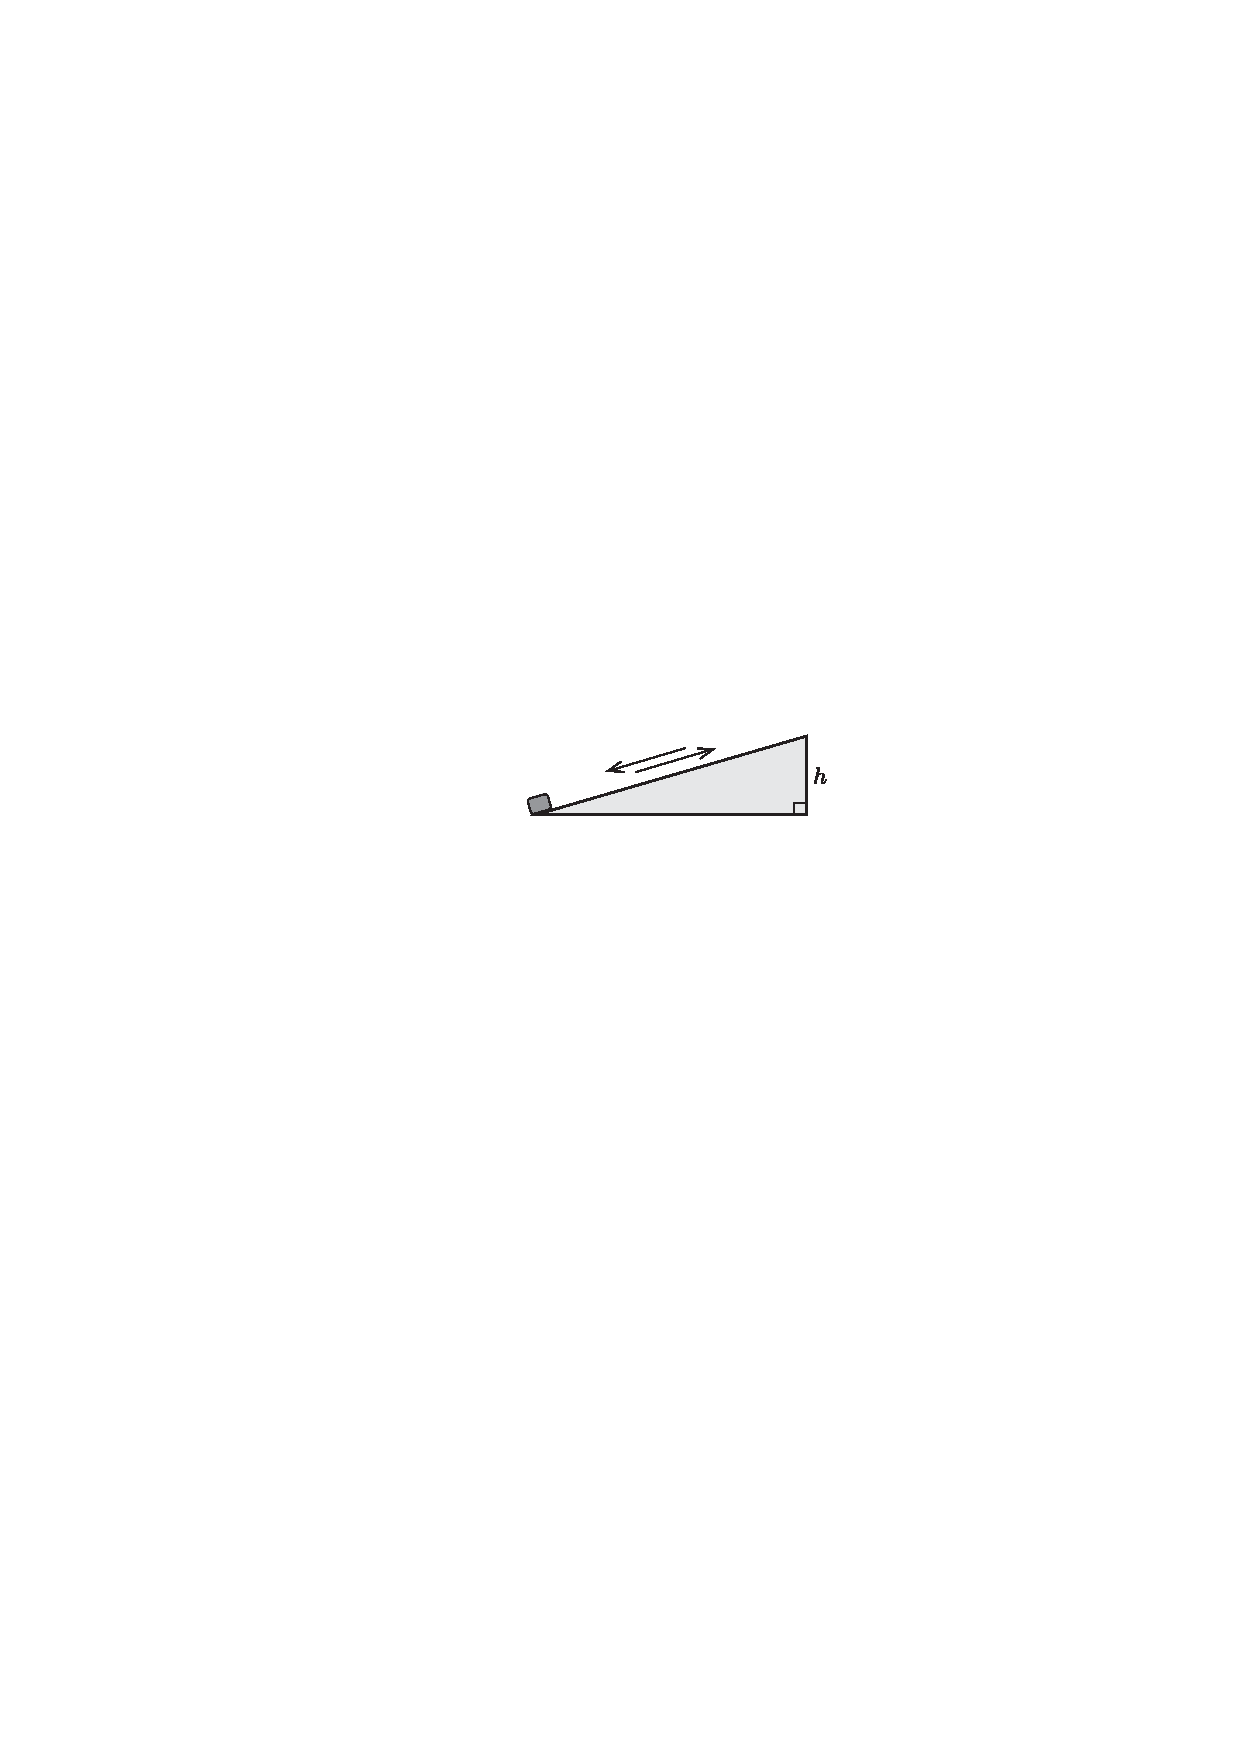
\includegraphics[width=0.5\linewidth]{incline}
\end{figure}
\vspace{8cm}\\
\noindent \textbf{ข้อ 2} วัตถุมวล \(M\) และ \(m\) เชื่อมติดกันด้วยสปริงเบาดังรูปและมีค่าสัมประสิทธิความเสียดทานจลน์ระหว่างพื้นผิวของมวลกับพื้นราบเท่ากับ \(\mu\) จงหาว่าแรงคงที่ ที่กระทำต่อมวล \(M\) ที่น้อยที่สุดที่จะทำให้มวล \(m\) ขยับมีค่าเท่าใด
\begin{figure}[h]
	\centering
	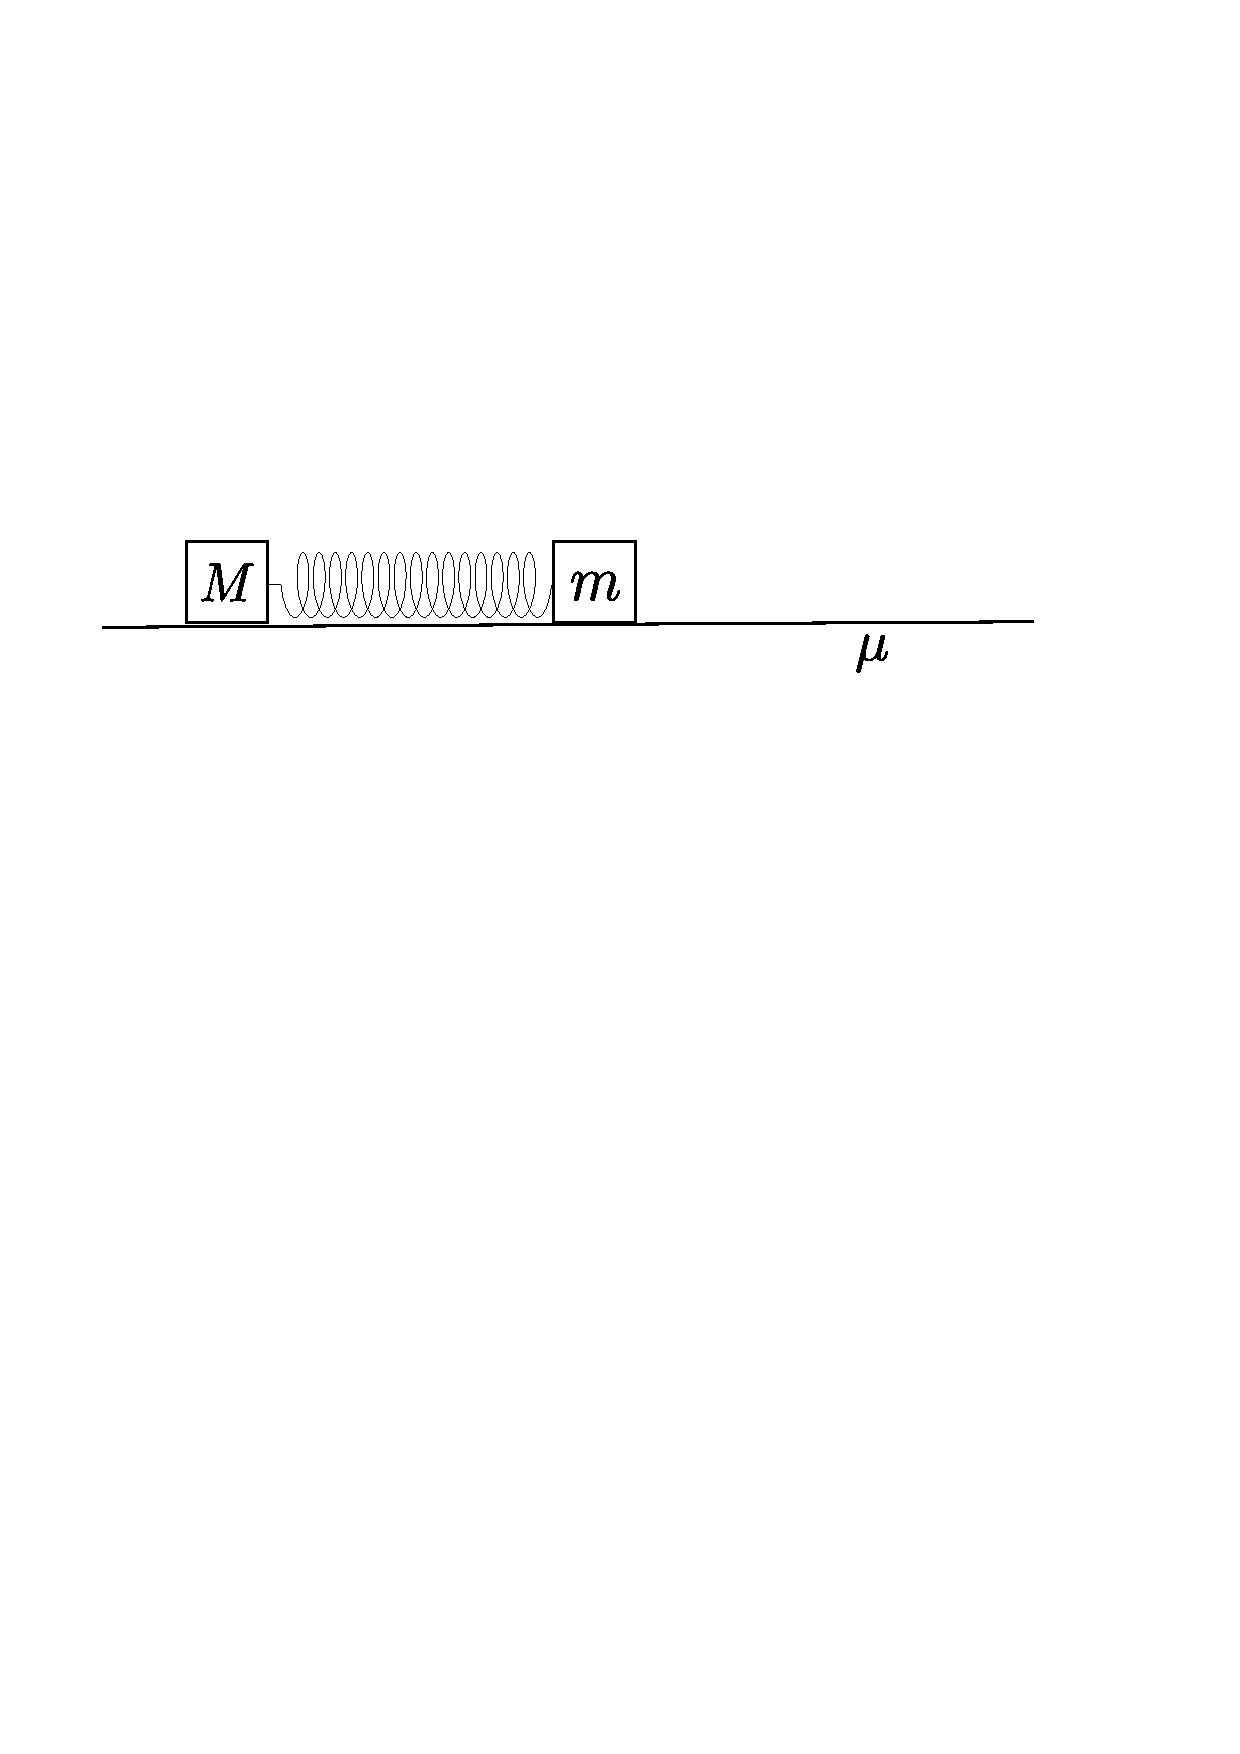
\includegraphics[width=0.5\linewidth]{two_mass_with_spring}
\end{figure}
\newpage

\begin{center}
	\textbf{{\Large เฉลย ข้อ 1}}
\end{center}
จาก
\begin{equation*}
	W=F\Delta x
\end{equation*}
งานลัพธ์เนื่องจากการเคลื่อนที่ \(n\) ครั้ง เท่ากับ
\begin{equation*}
	2nFL=2n(\mu mg\cos\theta)\left( \frac{h}{\sin\theta}\right) =\frac{2n(\tan\theta) mgh}{\tan\theta}=2nmgh
\end{equation*}
จากโจทย์ งานลัพธ์มีค่าเท่ากับ \(W\)
\begin{align*}
	W&=2nmgh\\
	\therefore h&=\frac{W}{2nmg}
\end{align*}
\newpage
\begin{center}
	\textbf{{\Large เฉลย ข้อ 2}}
\end{center}
สมมติให้ \(x\) เป็นระยะที่สปริงถูกบีบอัดและ \(k\) เป็นค่าคงตัวของสปริง
มอง \(m\)
\begin{equation}
	kx=\mu mg\label{eq:1}
\end{equation}
พิจารณามวล \(M\) โดยอาศัยทฤษฎีงาน-พลังงาน
\begin{align}
	W&=\Delta K\nonumber\\
	Fx-\mu Mgx&=\frac{1}{2}kx^2-0\nonumber\\
	F-\mu Mg&=\frac{1}{2}kx\label{eq:2}
\end{align}
นำสมการ (\ref{eq:1}) แทนในสมการ (\ref{eq:2})
\begin{align*}
	F-\mu Mg&=\frac{1}{2}\mu mg\\
	\therefore F&=\mu g\left( M+\frac{m}{2}\right)
\end{align*}
\end{document}